\myheader{Guía 5: Ecuaciones Diferenciales \\ y en Diferencias (Parte I)}

\begin{ejercicio}
    Sea un sistema LTI de tiempo discreto tal que la relación entre la salida y la entrada del mismo se puede escribir como:
    \begin{equation*}
        y(n) = \sum_{k=0}^{\infty} \alpha^{n-k} \left(x(k) + \beta x(k-1) + \gamma x(k-2)\right)
    \end{equation*}
    donde $|\alpha| < 1$ y $\beta, \gamma \in \R$.

    \inciso Obtener la respuesta al impulso del sistema y graficarla.
    
    \inciso Analizar la estabilidad del mismo.
    
    \inciso Determinar los valores de $\beta$ y $\gamma$ para que el sistema tenga las siguientes propiedades:
    \begin{itemize}
        \item Si $x(n) = (-1)^n$ para todo $n$ entonces $y(n) = 0$ para todo $n$.
        \item Si $x(n) = 1$ para todo $n$ entonces $y(n) = 1$ para todo $n$.
    \end{itemize}
\end{ejercicio}

\begin{ejercicio}
    Dado un sistema en tiempo discreto definido por la ecuación en diferencias 
    \begin{equation*}
        y(n) = x(n) + \frac{3}{4} y(n-1)
    \end{equation*}
    con condiciones de contorno
    \begin{align*}
    \inciso & y(-1) = 0 & \inciso & y(1) = 0 & \inciso & y(0) = 0 \\[.5em]
    \inciso & y(0) = 1 & \inciso & \lim_{n\rightarrow -\infty} y(n) = 0  & \inciso & \lim_{n\rightarrow +\infty} y(n) = 0
    \end{align*}
    se pide:
    \begin{itemize}
        \item Calcular el valor de la respuesta al impulso $h(n)$ del sistema en el intervalo $-5 \leq n \leq 5$
        \item Obtener una expresión cerrada de $h(n)$ para todo $n \in \mathbb{Z}$.
        \item Determinar si el sistema lineales, invariante ante desplazamientos, estables y causales.
    \end{itemize}
\end{ejercicio}
    
\begin{ejercicio}
    Dado un sistema en tiempo discreto definido por la ecuación en diferencias 
    \begin{equation*}
        y(n) = x(n) + \frac{1}{2} y(n-1)
    \end{equation*}
    con condiciones
    
    \inciso iniciales de reposo 

    \inciso finales de reposo

    \vspace*{1ex}

    \noindent se pide:
    \begin{itemize}
        \item Determinar si el sistema lineales, invariante ante desplazamientos, estables y causales. Establecer cómo se relacionan las condiciones de contorno con cada una de las propiedades del sistema.
        \item Calcular el valor de la respuesta a las señales $\delta(n-1)$ y $\delta(n+1)$ del sistema en el intervalo $-5 \leq n \leq 5$.
        \item Obtener una expresión cerrada de la respuesta a las señales $\delta(n-1)$ y $\delta(n+1)$ para todo $n \in \mathbb{Z}$.
    \end{itemize}
\end{ejercicio}
    
\begin{ejercicio}
    Demostrar que un sistema definido por ecuaciones en diferencias FIR siempre será lineal, invariante ante desplazamientos y estable. Determinar, además, qué condición debe cumplir un sistema de este tipo para ser causal.
\end{ejercicio}
    
\begin{ejercicio}
    Obtener la respuesta al impulso para el sistema definido por la ecuación diferencial 
    \begin{equation*}
        y(n) = x(n+1) + x(n) + x(n-1) + \frac{3}{4} y(n-1)
    \end{equation*}
    en condiciones inciales de reposo. 
\end{ejercicio}
    
\begin{ejercicio}
    Obtener la respuesta al impulso para el sistema definido por la ecuación diferencial 
    \begin{equation*}
        y(n) = x(n+1) + x(n) + x(n-1) + \frac{5}{4} y(n-1)
    \end{equation*}
    en condiciones finales de reposo. 
\end{ejercicio}
    
\begin{ejercicio}
    Implementar en \Keyboardsym una función que permita obtener la respuesta al impulso de una ecuación en diferencias para condiciones iniciales o finales de reposo.
\end{ejercicio}
    
\begin{ejercicio}
    Para el sistema descripto por la ecuación en diferencias $y(n) = \frac{1}{2} y(n-1) + x(n)$ con condiciones iniciales de reposo, se pide:
    
    \inciso Encontrar la expresión analítica de la salida $y(n)$ ante una entrada $x(n)$ aplicada a partir de $n = 0$.
    
    \inciso Encontrar a partir de la expresión anterior la salida que corresponde cuando la entrada es $x(n) = \delta(n)$. 
    
    \inciso Encontrar a partir de la expresión general de la salida del sistema, la salida que corresponde
    cuando la entrada es $x(n) = A e^{j\frac{\pi}{2}n}, n \geq 0$. A partir de esta expresión, y
    comparándola con la obtenida en el ejercicio anterior (c) discuta el significado de la respuesta permanente y de la transitoria. Grafique ambos tipos de respuesta en \Keyboard \hspace*{0.1em} y discuta cómo es mejor implementar la función que obtiene la salida del sistema, si mediante una convolución o un filtro recursivo.
\end{ejercicio}

\begin{ejercicio}
    Sea un sistema LTI y una señal $x(n)$ que satisface $x(n)= \delta(n) + \sum_{k=1}^M a_k x(n-k)$ donde $a_k \in \R$ para todo $k$. Sea $y(n)$ la salida del sistema cuando la entrada es $x(n)$.
    
    \inciso Determinar una ecuación en diferencias de $h(n)$ en función de $y(n)$ usando las propiedades básicas de un sistema LTI. 

    \inciso Si $y(n)$ es de duración finita, ¿qué se puede decir de la estabilidad del sistema?

    \inciso Si $y(n)$ es de duración infinita, obtener algún tipo de condición sobre $y(n)$ que asegure la estabilidad del sistema. 
\end{ejercicio}

\begin{ejercicio}
    Sea el sistema de tiempo continuo que, dada una entrada $x(t)$, la salida es $y(t) = \sum_{k=0}^{\infty} a_k x(t-kT)$ donde $a_k \in \R$ para todo $k$ y $T>0$. Este sistema puede modelar una situación donde existen una superposición de distintos ecos de la señal de entrada.

    \inciso Determinar si el sistema es LTI y, en caso afirmativo, determinar la respuesta al impulso.

    \inciso ¿Cuáles son las condiciones que en general deben cumplir los valores de $a_k$ (las amplitudes de
    los ecos) para que el sistema sea estable? Con este resultado, analizar el caso en que $a_k = \alpha^k$ con $\alpha \in \R$.

    \inciso Asumiendo que $a_k = \alpha^k$ con $|\alpha| < 1$, obtener un sistema que recupere la entrada $x(t)$ a partir de la salida $y(t)$ con ecos. Determinar, de ser posible, la ecuación en diferencias a coeficientes constantes que implementa el mismo. 
\end{ejercicio}

\begin{ejercicio}
    Sea la señal $x(t)$ cuya transformada de Fourier es $X(j\omega) = u(\omega - W_1) - u(\omega - W_2)$, con $W_1 < W_2$ y sea 
    \begin{equation*}
        y(t) = \frac{dx(t)}{dt} * x(t) + x(t)
    \end{equation*}
    Obtener $\int_{-\infty}^{\infty} |y(t-\alpha)|^2 dt$ donde $\alpha \in \R$.
\end{ejercicio}

\begin{ejercicio}
    Sea un sistema LTI cuya entrada es $x(n)$ y salida es $y(n)$. La relación entre la entrada y salida es:
    \begin{equation*}
        y(n) - \alpha y(n-1) = \sum_{k=-\infty}^{\infty} x(k) z(n-k) - x(n)
    \end{equation*}
    donde $z(n)$ es una secuencia cuya transformada de Fourier existe. 

    \inciso Encontrar la respuesta en frecuencia del sistema con $\alpha = \frac{1}{2}$. 

    \inciso Asumiendo que $z(n) = \beta^n u(n) + \delta(n)$ con $\beta = \frac{1}{3}$, encontrar la respuesta al impulso del sistema.
\end{ejercicio}

\begin{ejercicio}
    Sea un sistema LTI en tiempo discreto dado por:
    \begin{equation*}
        y(n) = \sum_{k=-\infty}^{n-1} \alpha^{n-k} \left( x(k - \beta_1) + x(k - \beta_2) \right),\; |\alpha| < 1, \; \beta_1, \beta_2 \in \mathbb{Z}\; \beta_2 > \beta_1
    \end{equation*}

    \inciso Determinar la respuesta al impulso $h(n)$ del sistema y la estabilidad del mismo. 

    \inciso Encontrar una ecuación en diferencias recursiva para el sistema.
\end{ejercicio}

\begin{ejercicio}
    Sea un sistema LTI en tiempo discreto causal con entrada $x(n)$ y salida $y(n)$ definido por el siguiente \emph{par} de ecuaciones diferenciales:
    \begin{align*}
        y(n) + \frac{1}{4} y(n-1) + w(n) + \frac{1}{2} w(n-1) &= \frac{2}{3} x(n) \\
        y(n) - \frac{5}{4} y(n-1) + 2w(n) - 2 w(n-1) &= -\frac{5}{3} x(n)
    \end{align*}
    \inciso Obtener la respuesta en frecuencia y la respuesta al impulso del sistema.
    
    \inciso Obtener una única ecuación en diferencias que relacione $x(n)$ con $y(n)$.
\end{ejercicio}

\begin{ejercicio}
    Un motor paso-a-paso puede modelarse a través del siguiente circuito:
    \begin{center}
        \parbox{0.5\textwidth}{
            \begin{circuitikz}[scale=0.8, transform shape, american voltages]
    \draw
    (0,0) to [american current source, l^=$i(t)$] (0,4)
    to (2,4)
    to [R, l^={\parbox{1.2cm}{
        \begin{center}
            $R_1$ \\ $100\;\Omega$    
        \end{center}
        }}] (2,0)
    to (0,0) ;
    \draw (2, 4) to [R, l_={$R_2$}] (6,4)
    to [L, l_={\parbox{1.2cm}{
        \begin{center}
            $L_1$ \\ $50\;\mu\mathrm{H}$    
        \end{center}
        }}, v^=$v_L(t)$] (6,0)
    to (2,0) ;

    \draw[->, thick] (3.3, 4.5) -- (4.6, 4.5);
    \node at (3.9, 4.8) {$i_1(t)$};
\end{circuitikz}
        }
    \end{center}
    
    En el mismo, el motor (representado por la inductancia $L_1$) se alimenta de una fuente de corriente $i(t)$. La ecuación de la corriente $i_1(t)$ que circula por el mismo se puede escribir como:
    \begin{equation*}
        i(t) = \frac{v_L(t)}{R_1} + \left(1 + \frac{R_2}{R_1}\right) i_1(t)
    \end{equation*}
    en donde la tensión $v_L(t) = L_1 \frac{d i_1(t)}{dt}$ es la tensión en los bornes de la inductancia. La fuente de corriente $i(t)$ entrega una corriente periódica de la siguiente forma:
    \begin{center}
        \parbox{0.5\textwidth}{
            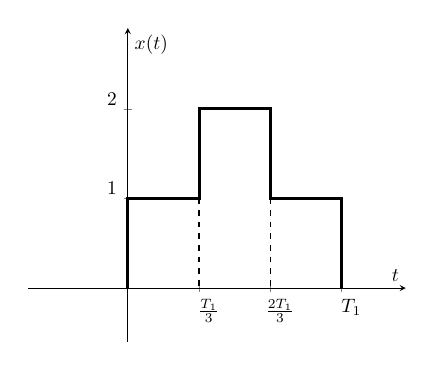
\begin{tikzpicture}[scale=0.7,transform shape]
    \begin{axis}[
    	axis y line=center,
    	axis x line=middle,
    	xlabel=$t$,ylabel=$x(t)$,
    	xmin=-1.4,xmax=3.9,
    	ymin=-0.6,ymax=2.9,
		xtick={0,1,2,3},
		xticklabels={0, $\frac{T_1}{3}$,$\frac{2T_1}{3}$,$T_1$},
    	xticklabel style = {xshift=5},
    	yticklabel style = {yshift=5},
    	]
    	\addplot[
    	black,
    	ultra thick
    	] coordinates {
    	    (0,0) (0,1) (1,1) (1,2)
    	    (2,2) (2,1) (3,1) (3,0)
    	};
		\addplot[
    	black,
    	thick,
		dashed
    	] coordinates {
    	    (1,1) (1,0)
    	};
		\addplot[
    	black,
    	thick,
		dashed
    	] coordinates {
    	    (2,1) (2,0)
    	};
    \end{axis}
\end{tikzpicture}

        }
    \end{center}
    \inciso Determinar la respuesta en frecuencia del sistema donde la entrada es $i(t)$ y la salida es $v_L(t)$.

    \inciso Determinar la representación en serie de Fourier de $i(t)$ y $v_L(t)$.

    \inciso Si se desea que la amplitud de la quinta armónica de la tensión en los bornes del inductor no supere los $10\;\mathrm{mV}$ dado que el motor debe funcionar cerca de un equipo sensible a la interferencia, determinar el valor de $R_2$ que garantiza eso. 
\end{ejercicio}

